\documentclass[xcolor={dvipsnames},pdf, hyperref={colorlinks=true, citecolor=ForestGreen, linkcolor=BlueViolet, urlcolor=Magenta}, handout]{beamer}
\usetheme{Frankfurt}  
\usecolortheme{whale}
\usepackage{tikz} 
\usepackage{graphicx}
\usepackage{dsfont}
\usepackage{hyperref}
\usepackage{alltt}
\usepackage{enumerate}
\usepackage{amsthm}
\theoremstyle{definition}
\newtheorem{exmp}{Example}[section]
\usepackage{verbatim}               % useful for \begin{comment} and \end{comment}
\usepackage{eurosym}                % used for euro symbol
\usepackage{caption} 
\usepackage{graphicx}
\usepackage{adjustbox}
\graphicspath{{Figures/}}
\usepackage{subcaption}
\usepackage{color}
\usepackage{float}
\usepackage{amssymb}
\usepackage{sgamevar}
\usepackage{remreset}% tiny package containing just the \@removefromreset command
\makeatletter
\@removefromreset{subsection}{section}
\makeatother
\setcounter{subsection}{1}

\newcommand{\defn}[1]{\textbf{#1}}


%Instructor version
\newcommand{\blank}[0]{}
\newcommand{\ddp}[1]{{\textcolor{ForestGreen}{#1}}} 
\newcommand{\dd}[1]{{\underline{\textcolor{ForestGreen}{#1}}}}

%Student version
%\newcommand{\blank}[0]{\vspace{2em}}
%\newcommand{\dd}[1]{\underline{\hspace{3cm}}} 
%\newcommand{\ddp}[1]{}

\addtobeamertemplate{navigation symbols}{}{%
	\usebeamerfont{footline}%
	\usebeamercolor[fg]{footline}%
	\hspace{1em}%
	\insertframenumber/\inserttotalframenumber
}


\section{Monopolistic Competition}

%% preamble
\title{Monopolistic Competition and Oligopoly}
\author{David A. D\'iaz}
\institute{UNC Chapel Hill}
\date{}

\AtBeginSection[] %Section links on slides

\begin{document} 
	
	\begin{frame}
		
		\titlepage
		
	\end{frame}


\begin{frame}{Monopolistic Competition}
\begin{itemize}
	\item 	\defn{Monopolistic Competition:} A market structure in which many firms sell products that are similar but not identical.
	
	Monopolistic competition arises in markets with the following attributes:
	\begin{enumerate}
		\item Many sellers \ddp{Many firms competing for the same group of customers.}
		\item Product differentiation \ddp{Product produced is at least slightly different than other firms $\Rightarrow$ Downward sloping demand.}
		\item Free entry and exit \ddp{$\Rightarrow \Pi = 0$.}
	\end{enumerate}
\end{itemize}
\end{frame}

\begin{frame}{Monopolistic Competition}
\begin{itemize}
	\item 	In the short-run, a firm in a monopolistically competitive market chooses its optimal quantity and price just like a monopolist: Find the quantity where \dd{$MR$} and \dd{$MC$} intersect and trace up to the \dd{demand} curve to find the price. 
	\item The only difference here is the slope of the demand curve: Because consumers in a monopolistically competitive market have numerous substitutes for the product each firm sells, the demand curve is more \dd{elastic}. 
\end{itemize}
\end{frame}

\begin{frame}{Monopolistic Competition}
		\begin{figure}[b]
		\centering
		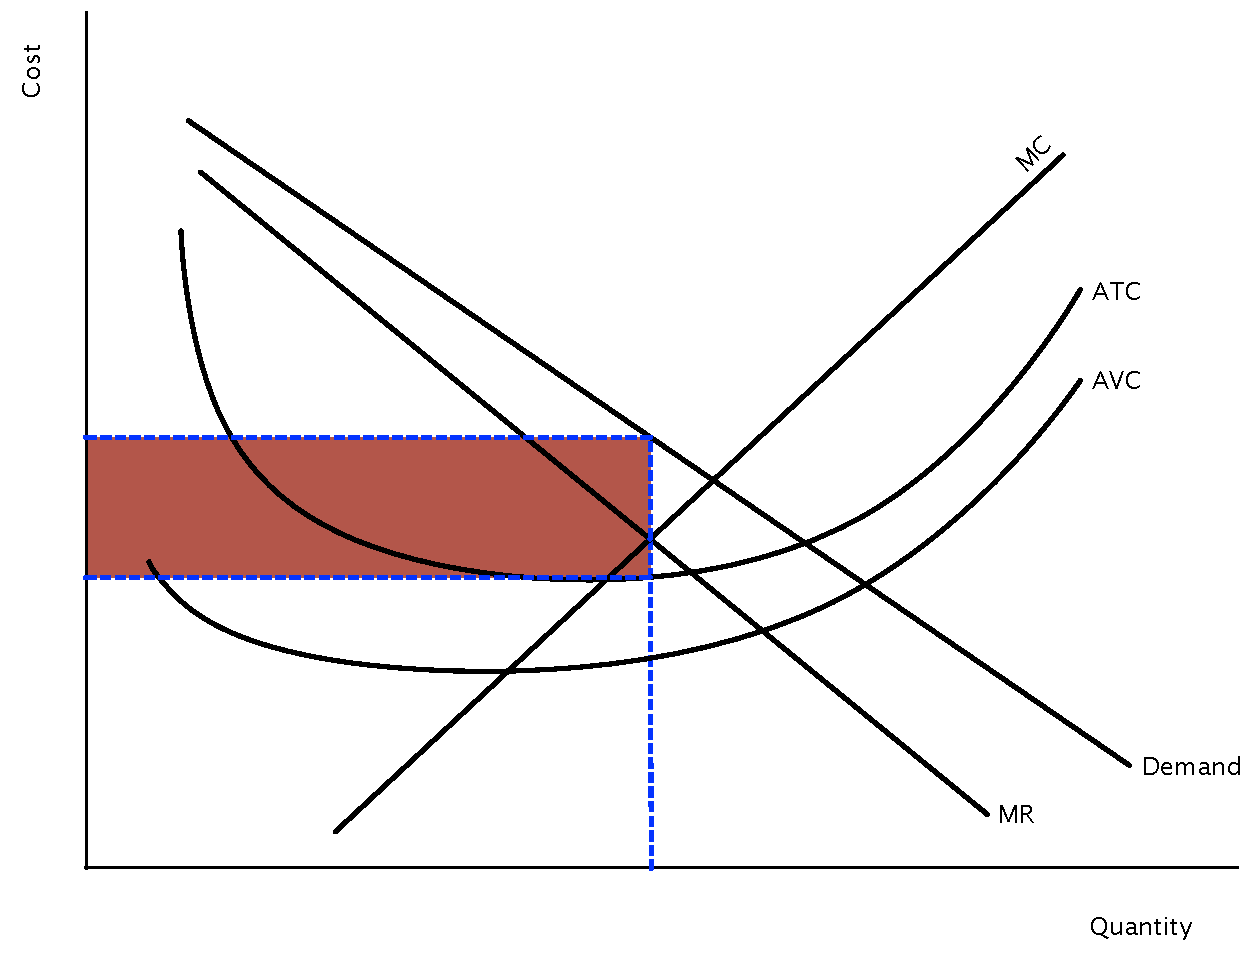
\includegraphics[scale=.40]{plot80.pdf}
		\caption{Monopolistic Competition in the Short-run}
	\end{figure}
\end{frame}

\begin{frame}{Monopolistic Competition}
	\begin{itemize}
		\item 	Because of the markup over marginal costs, some consumers who value the good more than the marginal cost but less than the price will be deterred from purchasing it. 
		\item As such, the welfare analysis is equivalent to that of a monopolistic firm.
	\end{itemize}
\end{frame}

\begin{frame}{Monopolistic Competition}
	
	\begin{figure}[b]
		\centering
		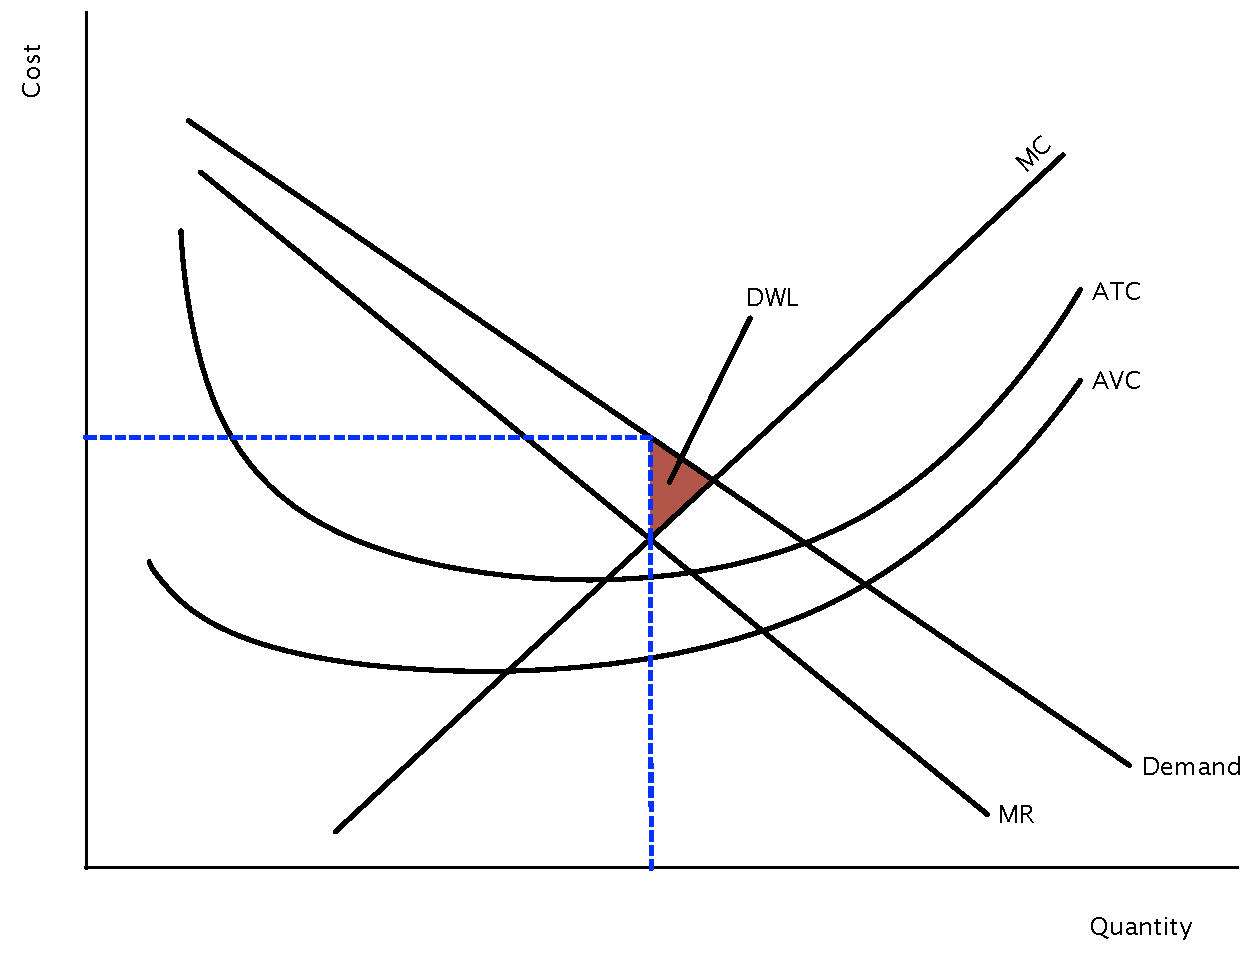
\includegraphics[scale=.40]{plot82.pdf}
		\caption{Monopolistic Competition and Welfare}
	\end{figure}
\end{frame}

\begin{frame}{Monopolistic Competition}
	\begin{itemize}
		\item 	Due to entry and exit, firms in markets characterized by monopolistic competition make \dd{zero (normal) profit} in the long run. 
		\item If firms in the industry are making profit, then other firms will enter the market. 
	
	\end{itemize}
\end{frame}

\begin{frame}{Monopolistic Competition}
	\begin{itemize}
	
		\item In this case, the demand faced by \textit{each} firm will \dd{decrease} since the number of products to choose from has increased. Moreover, each demand curve becomes \dd{more} elastic.
		\item If firms in the industry are making a loss, then firms will exit the market. 
		\item In this case, the demand faced by \textit{each} firm remaining will \dd{increase} since the number of products to choose from has decreased. Moreover, each demand curve becomes \dd{less} elastic.
	\end{itemize}
\end{frame}

\begin{frame}{Monopolistic Competition}
	\begin{itemize}
		\item 	The long run condition is that at the profit maximizing quantity, the demand curve and the average total cost curve are \dd{tangent}.
		\item Just like in a market with a monopoly, firms in monopolistically competitive markets charge a price that is \dd{greater} than the marginal cost. 
		\item Just like perfectly competitive markets, the process of entry and exit means that for firms in a monopolistically competitive market the long run the price is \dd{equal} to the average total cost. 
	\end{itemize}
\end{frame}

\begin{frame}{Monopolistic Competition}
	\begin{itemize}
		\item However, unlike firms in perfect competition, firms in a monopolistically competitive market do not produce at the \dd{social optimum} in the long run.
		\item The difference between the efficient scale and the quantity produced is called \dd{excess capacity}.
	\end{itemize}
\end{frame}


\begin{frame}{Monopolistic Competition}
	
\begin{figure}
	\centering
	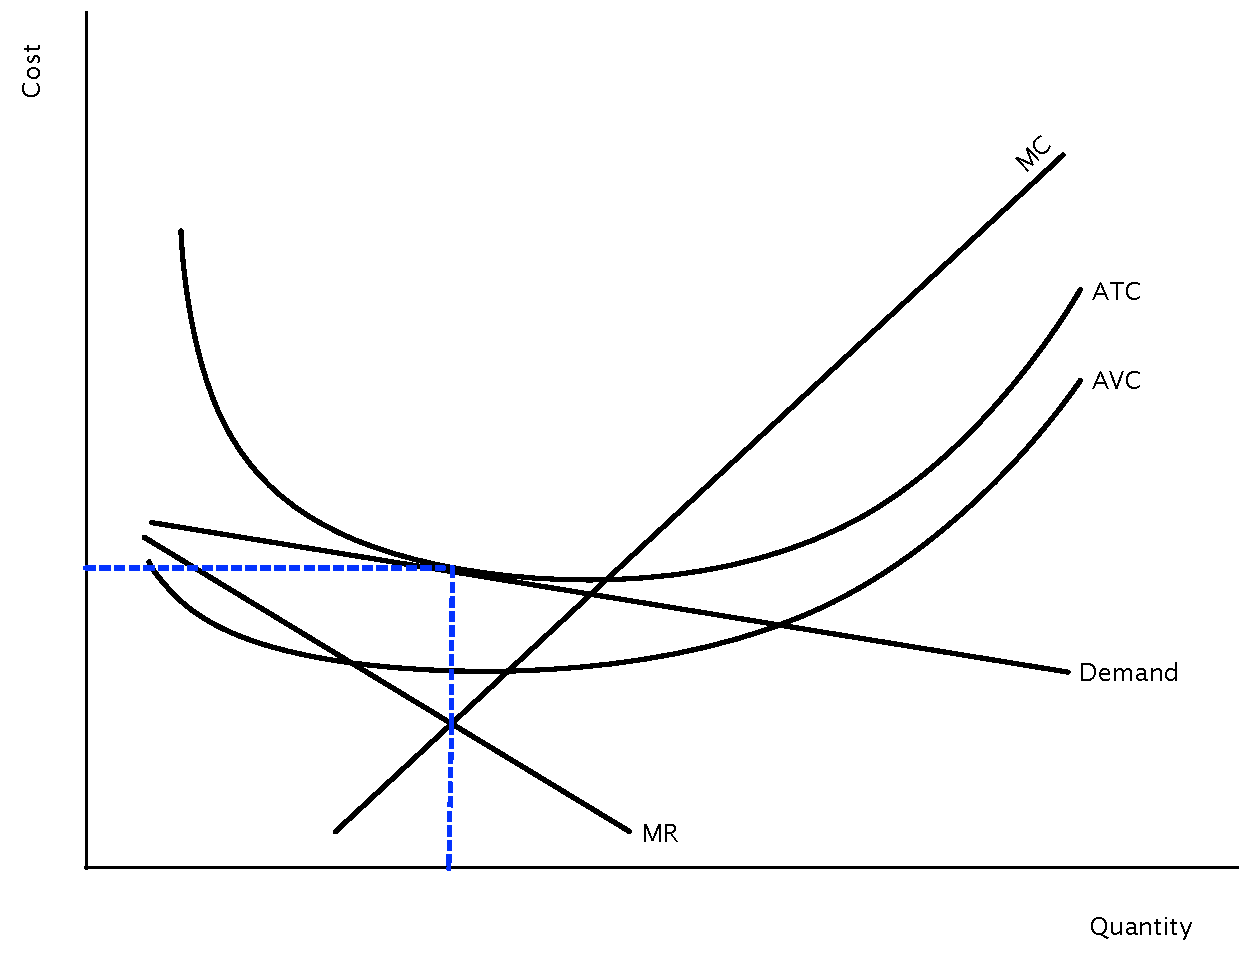
\includegraphics[scale=.40]{plot81.pdf}
	\caption{Monopolistic Competition in Long-run}
\end{figure}
\end{frame}



\begin{frame}{Monopolistic Competition}
Externalities associated with entry:
\begin{enumerate}
	\item Product-variety externality: New firms in the market leads to more differentiated products $\Rightarrow$ Increased surplus to consumers (positive externality)
	\item Business stealing externality: New firms steal existing customers and profits from existing firms (negative externality)
\end{enumerate}

\end{frame}

\section{Oligopoly}


\begin{frame}{Oligopoly}
\begin{itemize}
	\item 	
	\defn{Oligopoly:} A market structure in which only a few sellers offer similar or identical products.
	\item Due to the interdependence of the firms in an oligopoly, we will turn to concepts from elementary \textbf{game theory} (the study of how people behave in strategic interactions) in order to analyze how these firms behave. 
	
	
\end{itemize}
\end{frame}

\begin{frame}{Oligopoly}
	\scriptsize
\begin{exmp} Table \ref{diamonds} shows the $ATC$ and demand for diamonds. A large share of the world's supply of diamonds comes from Russia and South Africa. Suppose the two countries decide to work together in order maximize total profits. What would be the price and quantity? If they split production evenly, how much would Russia produce and what would be its profits?
	
		\begin{table}[H]
		\centering
		\caption{Demand Schedule}
		\label{diamonds}
		\begin{tabular}{  c| c | c | c| c| c| c}        
			
			Price & Quantity & ATC & TC & MC & TR &  MR  \\
			\hline
			\$8,000 & 5,000 & \$1,000 & \ddp{5,000,000} & \ddp{---} & \ddp{40,000,000} & \ddp{---}\\
			\$7,000 & 6,000 & \$1,000  & \ddp{6,000,000} & \ddp{1,000} & \ddp{42,000,000} & \ddp{2,000}\\
			\$6,000 & 7,000 & \$1,000  & \ddp{7,000,000} & \ddp{1,000} & \ddp{42,000,000} & \ddp{0}\\
			\$5,000 & 8,000 & \$1,000  & \ddp{8,000,000} & \ddp{1,000} & \ddp{40,000,000} & \ddp{--2,000}\\
			\$4,000 & 9,000 & \$1,000 & \ddp{9,000,000} & \ddp{1,000} & \ddp{36,000,000} & \ddp{--4,000}\\
			\$3,000 & 10,000 & \$1,000 & \ddp{10,000,000} & \ddp{1,000} & \ddp{30,000,000} & \ddp{--6,000}\\
			\$2,000 & 11,000 & \$1,000 & \ddp{11,000,000} & \ddp{1,000} & \ddp{22,000,000} & \ddp{--8,000}\\
			\$1,000 & 12,000 & \$1,000  & \ddp{12,000,000} & \ddp{1,000} & \ddp{12,000,000} & \ddp{--10,000}\\
			
		\end{tabular}
	\end{table} 
	
\pause	\ddp{Under collusion, countries act as a monopolist and produce as long as $MR\ge MC$. $Q^* = 6,000$ at $P^* = 7,000$. $\Pi = (7,000 - 1,000) \times 3,000 = \$18$M for each nation.}

	
\end{exmp}
\end{frame}



\begin{frame}{Oligopoly}
	\begin{exmp}
	What would happen to each nation's profit if Russia decided to increase their production by 1,000 and South Africa stuck to the original agreement? What would happen if they both increased their production by 1,000?
\end{exmp}

\ddp{If Russia deviates, ($P^*,Q^*) = (\$6,000, 7,000)$. $\Pi_R = (\$6,000 - 1,000) \times 4,000 = \$20$M. \\
	SA's profit is $\Pi_{SA} = (\$6,000 - 1,000) \times 3,000 = \$15$M. \\ If they both deviate,  ($P^*,Q^*) = (\$5,000, 8,000)$. $\Pi = (\$5,000 - 1,000) \times 4,000 = \$16,000$ for each.}

\end{frame}

\begin{frame}{Oligopoly}
\begin{itemize}
	\item 	\defn{Collusion:} An agreement among firms in a market about quantities to produce or prices to charge.
	\item \defn{Cartel:} A group of firms acting in unison.

\end{itemize}
\end{frame}

\begin{frame}{Oligopoly}
	\begin{itemize}

		\item As we saw in our example, the self-interest of each party drives each firm to produce more. Thus, the non-cooperative duopolist output is above the monopolist output level. 
		\item However, it will still be below that of a perfectly competitive firm's allocation. At some point of production, each firm will have no incentive to either increase or decrease their output level because they are already maximizing profit. 
		
	\end{itemize}
\end{frame}

\begin{frame}{Oligopoly}
\begin{itemize}
	\item \defn{Nash Equilibrium:} A situation where agents interacting with each other choose their best strategy given the strategies all other agents have chosen and can do no better by deviating.
	\item In summary, we have that when firms in an oligopoly individually choose their production levels to maximize profit, they produce a quantity \dd{greater} than that produced by a monopoly and \dd{less} than that produced under perfect competition. 
	\item Additionally, the oligopoly price is \dd{lower} than that of a monopoly and \dd{greater} than the competitive price.
\end{itemize}
\end{frame}

\begin{frame}{Oligopoly}
	\begin{exmp}
		\small
	Consider the utility gained by Jack and Jill as a result of their decisions to either snitch or keep mum. This is detailed in the table below.
	
\renewcommand{\gamestretch}{1.5}
\sgcolsep=25pt
\begin{figure}[h]\hspace*{\fill}%
	\begin{game}{2}{2}[Jack][Jill] 
		\>  Snitch \> Keep Mum \\
		Snitch \> $10, 10$ \> $30, 0$ \\
		Keep Mum \> $0, 30$ \> $20, 20$
	\end{game} 
	\hspace*{\fill}%
\end{figure}
	
	
\end{exmp} 
\end{frame}

\begin{frame}{Oligopoly}
\begin{itemize}
	\item 	Jack is the \dd{row} player and Jill the \dd{column} player.
	\item Jack's ``payoff'' is the first number in each box, while Jill's is the second. For example, if Jack decides to snitch and Jill keeps mum, Jack's payoff is \dd{30} and Jill's payoff is \dd{0}.
\end{itemize}
\end{frame}

\begin{frame}{Oligopoly}
	\begin{itemize}

		\item Let's look at this game from Jack's perspective: 
		\begin{itemize}
			\item If Jill snitches, he is better off \dd{snitching} as well since \dd{$10 > 0$}. We call this his \dd{best response}. 
			\item If Jill keeps mum, then Jack is still better off snitching since $30>20$. 
			\item No matter what Jill does, Jack is better off snitching. This type of strategy is referred to as a \dd{dominant strategy}. 
		\end{itemize}
	
	\end{itemize}
\end{frame}

\begin{frame}{Oligopoly}
	\begin{itemize}
		\item \defn{Dominant Strategy:} A strategy that is best for a player in a game regardless of the strategies chosen by other players.
		\item A similar analysis for Jill shows that her dominant strategy is to snitch as well. Thus, both parties end up snitching and receive payoffs of 10 and 10, respectively. This outcome is a \dd{Nash equilibrium}.   
	\end{itemize}
\end{frame}

\begin{frame}{Oligopoly}
	\begin{exmp}
	\scriptsize
	Write out the game form of example 12.1, where Russia is the row player and South Africa is the column player. Does either country have a dominant strategy? If there is one, what is the Nash equilibrium of this game?
	
	\renewcommand{\gamestretch}{.75}
	\sgcolsep=25pt
	\begin{figure}[htb]\hspace*{\fill}%
		\begin{game}{2}{2}[Russia][South Africa] 
			\>  Q = 3,000 \> Q = 4,000 \\
			Q = 3,000 \> \ddp{18,18} \> \ddp{15,20}\\
			Q = 4,000 \> \ddp{20,15} \> \ddp{16,16}
		\end{game} 
		\hspace*{\fill}%
	\end{figure}

	
\end{exmp}

\pause 	\ddp{Nash eq. is where each produces 4,000 as each nation's dominant strategy is to produce this amount.}
\end{frame}

\begin{frame}{Oligopoly}
\begin{exmp}
\scriptsize	
	Consider the game below, detailing the payoffs to Dynaco and Synergy when they decide on the size of their research budget. Does either party have a dominant strategy? If so, what is it? What will be the outcome if this game is played once?
	
	\renewcommand{\gamestretch}{1.5}
	\sgcolsep=25pt
	\begin{figure}[htb]\hspace*{\fill}%
		\begin{game}{2}{2}[Dynaco][Synergy] 
			\>  Large  \> Small  \\
			Large  \> \$30M, \$20M \> \$70M, \$0 \\
			Small  \> \$0, \$30M \> \$50M, \$40M \\
		\end{game} 
		\hspace*{\fill}%
	\end{figure}
\end{exmp}

\pause \ddp{\scriptsize Dynaco's dominant strategy is to have a large budget. \\
	 Synergy has no dominant strategy, but since they know Dynaco will play large budget, their best response is to play large budget. 
	 \\ The Nash eq. is (large budget, large budget).\\}
\end{frame}

\begin{frame}{Oligopoly}
\begin{itemize}
	\item 	Do parties always defect? No. Cooperation between parties is made easier when games are repeated.
	\item This is usually achieved by specifying what each party will do in order to maximize the payoff to both parties. 
	\item If either one defects in one period, then the other party imposes some sort of penalty by switching strategies the next period (and potentially forever after). 
	\item As long as each player cares enough about future payoffs, then they will forgo a one-time gain from defection.
\end{itemize}
\end{frame}

\begin{frame}{Readings and Assignments}
\begin{itemize}
	\item Today: Mankiw Ch. 16 \& 17
	\item Next time: Mankiw 23
	\item Problem Set 4, section 1
\end{itemize}
\end{frame}

\end{document}